\section{Datasets}
\label{sec:datasets}

\begin{table}[t]
\centering
\caption{Datasets, their group, test-set size and number of classes $C$. FP is the baseline top-1, the mean over the nine backbone and fine-tuning strategy settings.}
\label{tab:datasets}
\setlength{\tabcolsep}{2.5pt}
\small
\begin{tabular}{llrrr}
\toprule
Dataset & Group & Test $N$ & $C$ & FP (\%) \\
\midrule
Aircraft & FG & 3{,}333 & 100 & 78.4 \\
Cars & FG & 8{,}041 & 196 & 82.7 \\
CUB & FG & 5{,}794 & 200 & 89.1 \\
Dogs & FG & 8{,}580 & 120 & 88.5 \\
Flowers & FG & 6{,}149 & 102 & 98.8 \\
Food & FG & 25{,}250 & 101 & 90.4 \\
iNat17 & FG & 95{,}986 & 5{,}089 & 68.7 \\
Moe & FG & 2{,}943 & 173 & 91.4 \\
NABirds & FG & 24{,}633 & 555 & 86.7 \\
Pets & FG & 3{,}669 & 37 & 92.3 \\
VegFru & FG & 116{,}931 & 292 & 93.2 \\
SoyAgeing & UFG & 4{,}950 & 198 & 44.2 \\
SoyGene & UFG & 11{,}143 & 1{,}110 & 37.8 \\
SoyGlobal & UFG & 5{,}814 & 1{,}938 & 20.4 \\
SoyLocal & UFG & 600 & 200 & 27.1 \\
Cotton & UFG & 240 & 80 & 32.8 \\
\bottomrule
\end{tabular}
\end{table}


Test images are resized to 300 pixels and center-cropped to 224, and each context is evaluated with one inference seed.
CAL predictions aggregate cropped and flipped views, while its features come from the single test image.

\section{Feature properties}
\label{sec:diagnostics}

At W3/G128 we export the features after every block and the final logits of the baseline and quantized models for all 144 contexts.
Layer-wise similarity is the linear CKA~\cite{kornblith2019similarity} between the centered baseline and quantized features $X$ and $Y$,
\begin{equation}
  \mathrm{CKA}(X, Y) = \frac{\lVert X^{\top} Y \rVert_F^2}{\lVert X^{\top} X \rVert_F \, \lVert Y^{\top} Y \rVert_F}.
  \label{eq:cka}
\end{equation}
Depth is the block index divided by the number of positions (25 for Swin-B, 13 for the others), and mid depth pools all contexts at relative depths 0.45 to 0.55.
On $\ell_2$-normalized final features, $D_{\mathrm{intra}}$ is the mean cosine distance between images of one class and $D_{\mathrm{inter}}$ between images of two classes, each averaged with classes weighted equally.
Separability is $D_{\mathrm{inter}} - D_{\mathrm{intra}}$.
The H-score is $\mathrm{tr}\big(S_b (S_w + \lambda I)^{-1}\big)$ with between-class and within-class scatter $S_b$ and $S_w$ and $\lambda = 0.01\,\mathrm{tr}(S_w)/D$ for feature dimension $D$.

\section{Additional results}

\begin{table}[t]
\centering
\caption{Retention gap (FG $-$ UFG) at W3/G128 under alternative definitions: the mean and minimum over the nine settings, and the settings with a positive gap. Chance correction uses $(a_{\mathrm{Q}}-1/C)/(a_{\mathrm{FP}}-1/C)$. The worst leave-one-out row removes the dataset that lowers the mean gap most.}
\label{tab:robust}
\setlength{\tabcolsep}{3pt}
\small
\begin{tabular}{lrrr}
\toprule
Check & Mean & Min & Positive (of 9) \\
\midrule
Main analysis & 0.33 & 0.17 & 9 \\
Chance-corrected retention & 0.34 & 0.18 & 9 \\
Baselines below 15\% removed & 0.36 & 0.17 & 9 \\
Soybean datasets as one unit & 0.31 & 0.17 & 9 \\
Cotton alone & 0.27 & 0.08 & 9 \\
Soybean datasets alone & 0.34 & 0.18 & 9 \\
Leave out one dataset (worst) & 0.29 & 0.15 & 9 \\
\bottomrule
\end{tabular}
\end{table}


\begin{table}[t]
\centering
\caption{Retention gap (FG $-$ UFG) at W3/G128 before and after matching the baseline margin distributions, bin width 0.05. Red.: reduction of the gap. Overlap is the shared histogram mass; ESS is the lower of the two groups' matched-to-raw effective sample size.}
\label{tab:margin}
\setlength{\tabcolsep}{1.6pt}
\small
\begin{tabular}{llrrrrr}
\toprule
Backbone & Strategy & Raw & Matched & Red. (\%) & Overlap & ESS (\%) \\
\midrule
ViT-B/16 & FT & 0.212 & 0.042 & 80.0 & 0.26 & 23.4 \\
ViT-B/16 & FZ & 0.310 & 0.188 & 39.2 & 0.40 & 42.6 \\
ViT-B/16 & CAL & 0.268 & 0.118 & 55.9 & 0.24 & 29.6 \\
Swin-B & FT & 0.498 & 0.248 & 50.2 & 0.23 & 26.3 \\
Swin-B & FZ & 0.569 & 0.412 & 27.6 & 0.34 & 32.9 \\
Swin-B & CAL & 0.341 & 0.112 & 67.1 & 0.26 & 31.9 \\
BEiTv2-B & FT & 0.408 & 0.188 & 53.9 & 0.19 & 20.9 \\
BEiTv2-B & FZ & 0.184 & 0.078 & 57.4 & 0.37 & 34.1 \\
BEiTv2-B & CAL & 0.325 & 0.061 & 81.3 & 0.34 & 47.5 \\
\bottomrule
\end{tabular}
\end{table}


\begin{figure}[h]
  \centering
  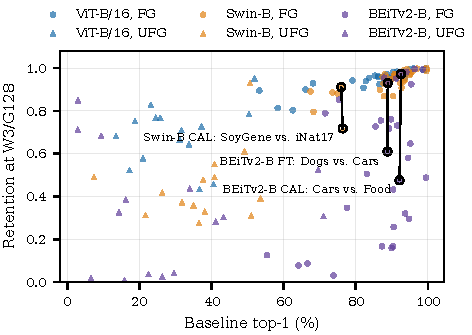
\includegraphics[width=\linewidth]{figures/accuracy_retention.pdf}
  \caption{Retention at W3/G128 against baseline top-1 for the \V{pooledN} contexts. Lines join three pairs from one setting with nearly equal baseline accuracy.}
  \label{fig:accuracy}
\end{figure}

\begin{table}[h]
\centering
\caption{Spearman correlation of each property with the difficulty score over the {\V{gridDatasets}} datasets. FP: baseline top-1. Sep.: separability. H: H-score. Norm: feature norm ratio P99/P50. All are measured on the baseline except the final-layer CKA between baseline and W3/G128 features.}
\label{tab:properties}
\setlength{\tabcolsep}{1.5pt}
\footnotesize
\begin{tabular}{llrrrrrrr}
\toprule
Backbone & Strategy & $q_{10}$ & FP & $C$ & Sep. & H & Norm & CKA \\
\midrule
ViT-B/16 & FT & $-$0.96 & $-$0.97 & 0.47 & $-$0.83 & $-$0.32 & 0.42 & $-$0.20 \\
ViT-B/16 & FZ & $-$0.93 & $-$0.91 & 0.30 & $-$0.83 & $-$0.25 & $-$0.90 & $-$0.48 \\
ViT-B/16 & CAL & $-$0.82 & $-$0.84 & 0.47 & 0.11 & 0.06 & 0.48 & $-$0.03 \\
Swin-B & FT & $-$0.87 & $-$0.82 & 0.48 & $-$0.73 & $-$0.56 & $-$0.39 & $-$0.51 \\
Swin-B & FZ & $-$0.97 & $-$0.98 & 0.36 & $-$0.80 & $-$0.15 & $-$0.81 & $-$0.31 \\
Swin-B & CAL & $-$0.65 & $-$0.67 & 0.49 & 0.10 & $-$0.43 & $-$0.10 & $-$0.19 \\
BEiTv2-B & FT & $-$0.53 & $-$0.45 & 0.03 & $-$0.44 & $-$0.27 & $-$0.19 & $-$0.35 \\
BEiTv2-B & FZ & $-$0.93 & $-$0.96 & 0.31 & $-$0.86 & $-$0.42 & 0.69 & $-$0.17 \\
BEiTv2-B & CAL & $-$0.80 & $-$0.72 & 0.21 & 0.27 & $-$0.09 & $-$0.04 & 0.25 \\
\bottomrule
\end{tabular}
\end{table}


The full grid and the paired W3/G128 exports come from separate evaluation runs of the same checkpoints.
On the \V{consistContexts} contexts present in both, baseline top-1 differs by at most \V{consistFp} points and W3/G128 top-1 by at most \V{consistQ} points.
With matching bin widths 0.025, 0.05 and 0.1, the reduction of the retention gap ranges from \V{reductionMinAll}\% to \V{reductionMaxAll}\%.
